\subsection{Klassifikation der endlichen Rotationsgruppen}
Für das folgende Kapitel nehmen wir an, dass wir $\dim V = 3$ und dass $W$ eine Ebene in $V$ ist. Wenn nun $R$ eine Rotation in $\mathcal{O}(W)$, dann kann $R$ zu einer Rotation in $\mathcal{O}(V)$ erweitert werden, indem wir $Rx=x$ für alle $x \in W^\perp$ setzten und eine Basis ${x_1,x_2,x_3}$ für $V$ wählen mit $x_1 \in W^\perp$, $x_2, x_3 \in W$. Dann wird $R$ durch die Matrix A repräsentiert.
$$A=\begin{pmatrix}
1 & 0 & 0 \\
0 & \cos{\theta} & -\sin{\theta} \\
0 & \sin{\theta} & \cos{\theta}
\end{pmatrix} $$ 
Zunächst wollen wir uns überlegen wie wir die zyklische Gruppe und die Diedergruppe ins dreidimensionale überführen können. Als erstes erweitern wir jede Rotation der zyklischen Gruppe im zweidimensionalen wie oben beschrieben, in eine Rotation im dreidimensionalen Raum und erhalten so die zyklische Gruppe im dreidimensionalen Raum, die wir mit $\mathcal{C}_3^n$ bezeichnen. 

Um auch die Diedergruppe ins dreidimensionale zu überführen, müssen wir uns nun damit befassen wie wir Spiegelungen im zweidimensionalen in den dreidimensionalen Raum überführen können. Wenn eine Spiegelung $S$ aus $\mathcal{W}$ ist, dann erweitern wir sie zu einer Rotation in $\mathcal{O}(V)$ und zwar zu einer Rotation $R$, um den Ursprung mit Winkel $\pi$. Die Spiegelgerade von $S$ wird die Rotationsachse von $R$, diese Beziehung wollen wir zeigen:
\begin{proof}
	Angenommen, dass $\dim V = 3$ und dass $W$ eine Ebene in $V$ ist. Sei $R \in V$ eine Rotation um den Winkel $\pi$. Alle Punkte die auf der Rotationsachse liegen sind Fixpunkte von $R$. Damit die Rotationsachse, die ehemalige Spiegelachse der Spiegelung $S$ sein kann, müssen die Fixpunkte der beiden Achsen übereinstimmen. Zunächst bestimmen wir die Fixpunkte von $R$:
	\begin{align*}
	E_R(1) &= \ker{(R-E)} \\
	&= \ker{\begin{pmatrix}
		-2 & 0 & 0 \\
		0 & \cos{\theta} - 1 & \sin{\theta} \\
		0 & \sin{\theta} & -\cos{\theta} -1
		\end{pmatrix}} \\
	&= \ker{\begin{pmatrix}
		1 & 0 & 0 \\
		0 & \sin{\theta}(\cos{\theta} - 1) & \sin^2{\theta} \\
		0 & \sin{\theta}(\cos{\theta} - 1) & (-\cos{\theta} -1)(\cos{\theta} + 1)
		\end{pmatrix}} \\
	&= \ker{\begin{pmatrix}
		1 & 0 & 0 \\
		0 & \sin{\theta}(\cos{\theta} - 1) & \sin^2{\theta} \\
		0 & 0 & -cos^2{\theta}-sin^2{\theta}+1
		\end{pmatrix}} \\
	&= \ker{\begin{pmatrix}
		1 & 0 & 0 \\
		0 & \sin{\theta}(\cos{\theta} - 1) & \sin^2{\theta} \\
		0 & 0 & 0
		\end{pmatrix}} \\
	&= \Span\left\{\begin{pmatrix} 0 \\
	(1 + \cos{\theta}) \\
	\sin{\theta}
	\end{pmatrix}\right\}
	\end{align*}
Jetzt überprüfen wir, ob $S$ in der Ebene die selben Fixpunkte besitzt, dass heißt wir überprüfen ob $Sx=x$ für alle $x$ aus der Fixpunktmenge von $R$ gilt. Sei $x = r(1+\cos{\theta},\sin{\theta})^T$ mit $r \in \mathbb{R}$.
	\begin{align*}
		Sx &= \begin{pmatrix}
			\cos{\theta} & \sin{\theta} \\
			\sin{\theta} & -\cos{\theta}
		\end{pmatrix}\begin{pmatrix}
		r(1 + \cos{\theta}) \\
		r\sin{\theta}
		\end{pmatrix} \\
		&=	\begin{pmatrix}
		r(1 + \cos{\theta})(\cos{\theta})+rsin^2{\theta} \\
		r(1 + \cos{\theta})\sin{\theta}+(- \cos{\theta})r\sin{\theta}
		\end{pmatrix} \\
		&=	\begin{pmatrix}
		r(1 + \cos{\theta}) \\
		r\sin{\theta}
		\end{pmatrix}
	\end{align*}
Somit haben wir gezeigt, dass die Fixpunkte der Rotation auch Fixpunkte der Spiegelung sind und damit die Rotationsachse mit der ursprünglichen Spiegelachse übereinstimmt.
\end{proof}
Wenn wir jede Abbildung in einer Diederuntergruppe $\mathcal{H}^n_2$ aus $\mathcal{O}(W)$ in eine Rotation aus $\mathcal{O}(V)$ erweitern, dann ist die resultierende Menge von Rotationen eine Untergruppe von $\mathcal{O}(V)$, welche isomorph zu $\mathcal{H}^n_2$ ist. Diese Untergruppe nennen wir auch Diedergruppe und bezeichnen sie mit $\mathcal{H}^n_3$. \textbf{(Übung 2.9)}
Nun wollen wir uns mit den Rotationsgruppen der Platonischen Körper beschäftigen. Wenn wir ein reguläres Polyeder um den Ursprung im dreidimensionalen Raum zentrieren, dann bilden die Rotationen aus $\OR{3}$ die das Polyeder wieder in sich überführen eine endliche Untergruppe von $\OR{3}$. Wir können auf die Art und Weise nur drei von einander unterscheidbare Untergruppen finden. Denn die Rotationsgruppen des Würfels und des Oktaeders enthalten die selben Elemente. Genauso verhält es sich mit dem Dodekaeder und dem Ikosaeder. Diesen Zusammenhang können wir uns geometrisch überlegen. Wenn wir die Mittelpunkte benachbarter Seitenflächen des Würfels miteinander verbinden dann erhalten wir ein in den Würfel einbeschriebenes Oktaeder. Das heißt, dass das Oktaeder unter den Elementen der Rotationsgruppe des Würfels invariant bleibt. Wir hätten auch nach dem selben Prinzip den Würfel in das Oktaeder einbeschreiben können. Bei dem Dodekaeder und dem Ikosaeder können wir ähnlich argumentieren. Schauen wir uns dem Zusammenhang in Abbildung \ref{fig:Duality_Dodek-Iso} an, wird er noch klarer. 
\begin{figure}[H]
\centering
\includegraphics[width=0.4\linewidth]{grafiken/Duality_Dodek-Iso}
\caption{Dualität der Platonischen Körper}
\label{fig:Duality_Dodek-Iso}
\end{figure}
Jetzt wollen wir uns genauer mit den Rotationsgruppen der Platonischen Körper befassen. Um die folgenden Gedankengänge leichter zu verstehen, kann die Webanwendung \href{http://www-stud.uni-due.de/~simibark/visualisierung-platonische-koerper}{Visualisierung Platonische Körper} genutzt werden.

Angenommen, dass ein Tetraeder am Ursprung des dreidimensionalen Raums ausgerichtet ist. Die Rotationsgruppe, die alle Abbildungen enthält die das Tetraeder wieder in sich überführen werden wir mit $\mathcal{T}$ bezeichnen. Nun müssen wir uns überlegen, welche Rotationen in dieser Untergruppe enthalten sind. Die Tetraedergruppe $\mathcal{T}$ enthält acht Rotationen um die Rotationsachsen zwischen einem Eckpunkt und dem Mittelpunkt der gegenüberliegenden Seite mit Rotationswinkeln $\frac{2}{3}\pi$ und $\frac{4}{3}\pi$, drei Rotationen um die Rotationsachsen zwischen den Mittelpunkten zweier gegenüberliegender Kanten mit Rotationswinkel $\pi$ und die Identität. Es gilt somit $| \mathcal{T} | = 4 \cdot 2 + 3 \cdot 1 + 1 = 12$.

Die Rotationsgruppe des Würfels bezeichnen wir mit $\mathcal{W}$. Die Würfelgruppe $\mathcal{W}$ enthält drei verschiedene Arten von Rotationen und die Identität. Zum einen enthält sie neun Rotationen mit den Winkeln $\frac{1}{2}\pi$ ,$\pi$ und $\frac{3}{2}\pi$ um die Rotationsachsen zwischen den Mittelpunkten zweier gegenüberliegender Seiten, acht Rotationen mit den Winkeln $\frac{2}{3}\pi$ und $\frac{4}{3}\pi$ um die Rotationsachsen zwischen zwei diagonal gegenüberliegenden Eckpunkten und zuletzt sechs Rotationen mit den Winkel $\pi$ um die Rotationsachse zwischen den Mittelpunkten zweier diagonal gegenüberliegender Kanten. Es gilt somit $| \mathcal{W} | = 3 \cdot 3 + 4 \cdot 2 + 6 \cdot 1 + 1 = 24$.

Die Rotationsgruppe $\mathcal{I}$ des Ikosaeders enthält 24 Rotationen um die Rotationsachsen zwischen zwei gegenüberliegenden Eckpunkten mit Rotationswinkel $\frac{2}{5}\pi$, $\frac{4}{5}\pi$, $\frac{6}{5}\pi$, $\frac{8}{5}\pi$, 20 Rotationen um die Rotationsachsen zwischen den Mittelpunkten zweier gegenüberliegender Seiten mit Rotationswinkel $\frac{2}{3}\pi$, $\frac{4}{3}\pi$, 15 Drehungen um die Rotationsachse zwischen den Mittelpunkten zweier gegenüberliegender Kanten mit Rotationswinkel $\pi$ und der Identität. Es gilt somit $| \mathcal{I} | = 15 \cdot 1 + 10 \cdot 2 + 6 \cdot 4 + 1 = 60$.

Wir haben nun die Rotationsgruppen der zyklischen Gruppe, Diedergruppe und aller regelmäßigen Polyeder bestimmt. Doch bevor wir mit der Klassifizierung der endlichen Rotationsgruppen beginnen können, müssen wir zunächst noch den Begriff des Pols einführen.

\begin{defi}[Pole]
	Wenn $T \in \mathcal{O}(V)$ eine Rotation ausgeschlossen der Identität $E$ ist, dann erhalten wir genau zwei Schnittpunkte der Rotationsachse mit der Einheitskugel um den Ursprung. Diese beiden Punkte nennen wir Pole. Die Menge aller Pole einer Untergruppe $\mathcal{G}$ von $\mathcal{O}(V)$ bezeichnen wir mit $\mathcal{P}$
\end{defi} 

Jetzt können wir die Menge der Pole zu den einzelnen Rotationsgruppen, die wir zuvor diskutiert haben, aufstellen und ihre Mächtigkeit ermitteln. Die zyklische Gruppe $\mathcal{C}^n_3$ enthält $n$ Rotationen, die alle dieselbe Rotationsachse besitzen. Daher besitzt die Polmenge $\mathcal{P}$ zu $\mathcal{C}^n_3$ genau zwei Elemente. Außerdem können wir festhalten, dass kein Pol durch eine Transformation aus $\mathcal{C}^n_3$ auf den anderen überführt wird, daher besitzt $\mathcal{P}$ zwei ein-elementige Bahnen. Wenn wir uns die Bahnformel zur Hilfe nehmen, können wir daraus die Ordnung der Stabilisatoren für die Pole ableiten. Diese kennen wir aus der linearen Algebra und lautet wie folgt:
$$ |G| = |G \circ p| \cdot |G_p| $$
Dabei ist $G \circ p = \{g \circ p | g \in G\}$, die Bahn von p und $G_p = \{g \in G | g \circ p = p \}$, der Stabilisator von p. 

Wenden wir diese nun auf unser Beispiel an, können wir aus der folgenden Gleichung die Ordnung des Stabilisators ableiten.
\begin{align*}
	 |\mathcal{C}_3^n| &= |\mathcal{C}_3^n \circ p| \cdot |{\mathcal{C}_3^n}_p| \Leftrightarrow\\
	 n &= 1 \cdot |{\mathcal{C}_3^n}_p|
\end{align*}
Jetzt wissen wir, dass die Ordnung des Stabilisators für einen Pol $n$ ist. Als nächstes betrachten wir die Pole der Diedergruppe $\mathcal{H}_3^n$. Diese Gruppe enthält $n$ Rotationen mit verschiedenen Rotationsachsen und eine Rotation, die orthogonal zu den anderen Rotationen steht, demnach enthält die Menge der Pole $\mathcal{P}$ der Gruppe $\mathcal{H}_3^n$ $2n+2$ Pole. Diese Pole kommen auf drei verschiedene Arten zustande. Zum einen erhalten wir Pole von Rotationsachsen die durch die Eckpunkte des Polygon gehen, dann erhalten wir Pole von Rotationsachsen durch die Mittelpunkte der Kanten des Polygons und Pole von der Rotationsachse der Transformationen der zyklischen Gruppe. Zur Veranschaulichung können wir uns die Abbildung angucken.
\begin{figure}[H]
\centering
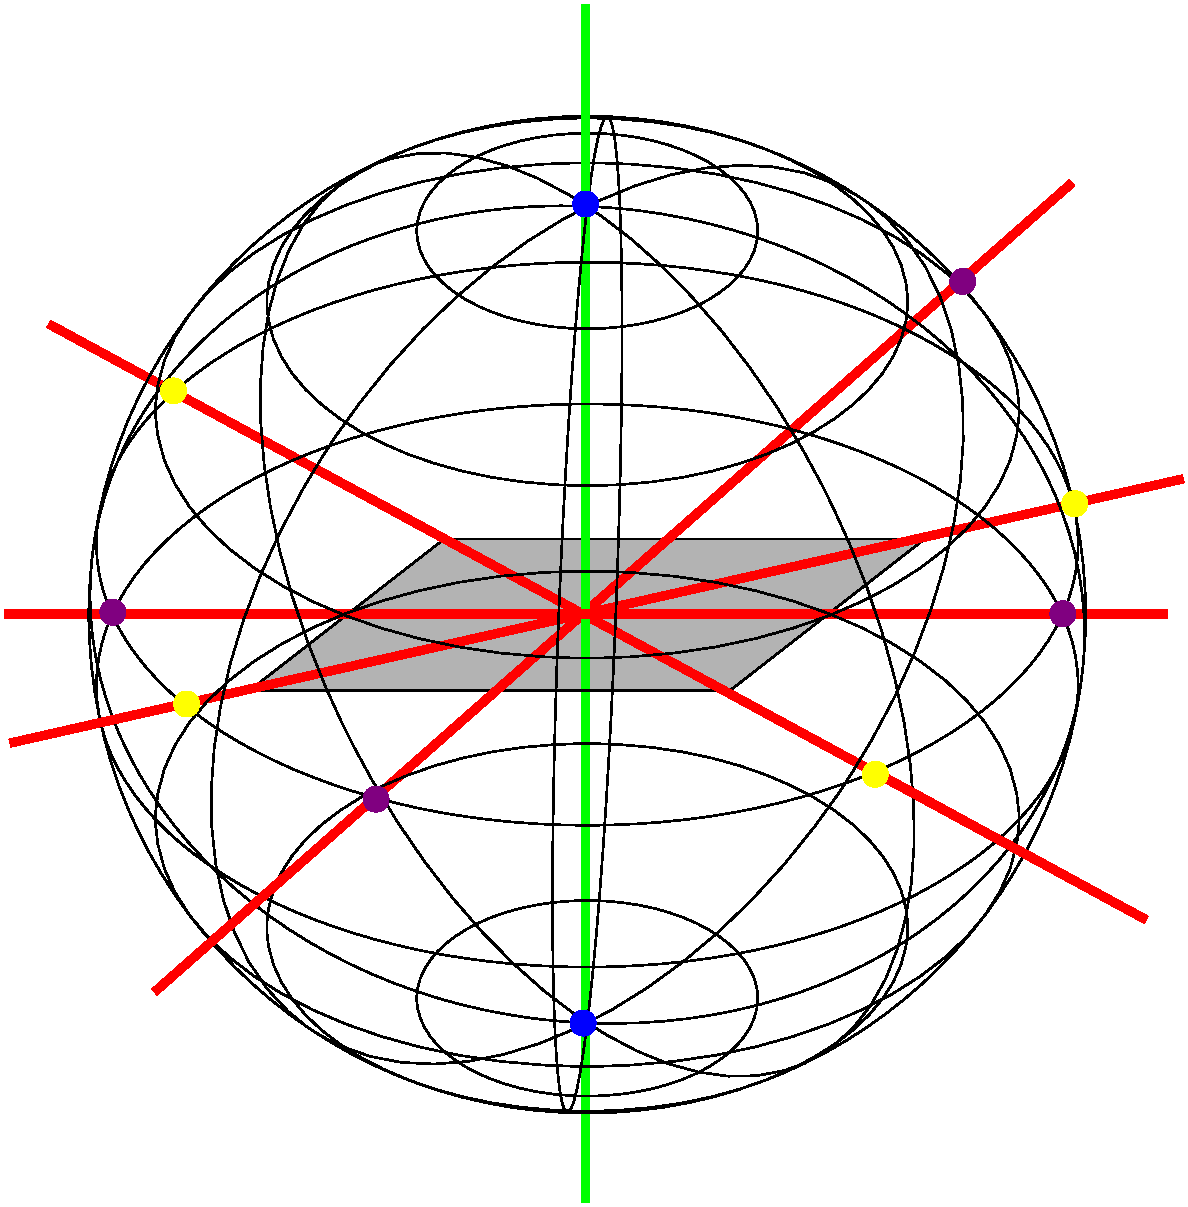
\includegraphics[width=0.5\linewidth]{grafiken/pole_diedergruppe}
\caption{Pole der Diedergruppe $\mathcal{H}_3^4$}
\label{fig:pole_diedergruppe}
\end{figure}
